% -*- TeX-engine: luatex -*-
\RequirePackage[l2tabu,orthodox]{nag}

\documentclass[paperwidth=60in,paperheight=36in,landscape]{baposter}
\usepackage[cmyk]{xcolor}
\definecolor{firedrake_red}{cmyk}{0.07,0.86,0.8,0.09}
\definecolor{purple}{cmyk}{0.51,0.91,0,0.34}
\definecolor{blue}{cmyk}{1,0,0,0.9}
\definecolor{black}{cmyk}{0,0,0,0.95}
\definecolor{red}{cmyk}{.15,1,0.9,0.1}
\definecolor{cyan}{cmyk}{1,0,0,0}
\definecolor{yellow}{cmyk}{0,0.15,0.87,0}
\usepackage[lined,commentsnumbered]{algorithm2e}
\usepackage{amsmath}
\usepackage{amssymb}
\usepackage{amsfonts}
\usepackage{mathtools}
\usepackage[final,letterspace=50,step=2,stretch=10]{microtype}
\microtypecontext{spacing=nonfrench}
\usepackage{url}
\usepackage{minted}
\usepackage{tikz}
\usepackage{tikz}
\usetikzlibrary{cd}
\usetikzlibrary{calc, positioning, trees, plotmarks}
\usetikzlibrary{shapes, shapes.geometric, decorations.pathreplacing, decorations.markings}
\usetikzlibrary{arrows, arrows.meta, chains, fit, backgrounds, scopes}

\usepackage{graphicx}
\usepackage[export]{adjustbox}

\graphicspath{{./\jobname.figures/}{../pictures/}}

\usepackage{booktabs}
\usepackage[most]{tcolorbox}
\usepackage{amsmath,amssymb}
\usepackage{cmbright}
\usepackage{fontspec}
\defaultfontfeatures{
  Ligatures = TeX,
  Scale = 1,
  Extension = .otf }
\setmainfont[
Numbers = {Monospaced, Lining},
UprightFont={*-Light},
ItalicFont ={*-Light Italic},
BoldFont ={*-Medium},
BoldItalicFont ={*-Medium Italic},]{FiraSans}
\setsansfont[
Numbers = {Monospaced, Lining},
UprightFont= *-Light,
ItalicFont = *-Light Italic,
BoldFont = *-Medium,
BoldItalicFont = *-Medium Italic,]{FiraSans}

\usepackage{ragged2e}

\begin{document}

\begin{poster}{
    grid=false,
    columns=6,
    colspacing=0.5em,
    textborder=faded,
    boxColorOne=white,
    headerColorOne=purple,
    borderColor=purple,
    headerFontColor=white,
    headerborder=open,
    textfont=\color{blue},
    headerfont=\bfseries\Large\scshape,
    eyecatcher=true,
    headershape=rounded,
    headershade=plain,
    background=none,
    headerheight=0.1\textheight,
  }
  {
    \begin{minipage}[c]{0.2\textwidth}
      {\raggedright
        
\includegraphics[height=0.8cm]{nyu-logo-left}
        \hskip10pt
        
\includegraphics[height=0.8cm]{nyu-logo-right}\\[0.5\baselineskip]

        
\includegraphics[height=1.5cm]{durham-logo}
        \par
      }
    \end{minipage}
  } 
  % Title
  {{\color{blue}\bfseries\scshape\fontsize{20}{22}\selectfont \texttt{PCPATCH}: topological construction of multigrid
      relaxation schemes\par}}
  % Authors
  {{\color{blue}\vspace{0.2em}\small\scshape Lawrence~Mitchell\\
      {\normalfont \texttt{lawrence.mitchell@durham.ac.uk}}
      \\[0.5em]
      {\footnotesize Patrick~E.~Farrell \quad Matthew~G.~Knepley \quad Florian
        Wechsung\\
        {\normalfont \texttt{patrick.farrell@maths.ox.ac.uk} \quad
          \texttt{knepley@buffalo.edu} \quad \texttt{wechsung@nyu.edu}}}}}
  % University logo
  {%
    \begin{minipage}[c]{0.2\textwidth}
      
      {\flushright
        
\includegraphics[height=0.8cm]{buffalo-logo}\\[0.5\baselineskip]

        
\includegraphics[height=1.5cm]{oxford-logo}
        \par}
    \end{minipage}
    
  }%
  \begin{posterbox}[name=introduction,span=2,column=0,row=0, height=1]{Block
      Jacobi multigrid smoothers}
    \vspace{0.25\baselineskip}
    {\centering\Large\bfseries H(curl) multigrid\strut\par}
    \vspace{-0.75\baselineskip}
    \begin{equation*}
      (u, v) + \alpha(\nabla \times u, \nabla \times v) = (f, v)
    \end{equation*}
    
    \begin{minipage}[t]{0.66\linewidth}
\begin{minted}{text}
-mg_levels_pc_type patch
-mg_levels_pc_patch_construct_type star
-mg_levels_pc_patch_construct_dim 0
\end{minted}      
      \begin{tabular}{cc|ccccc}
        \toprule
        levels & DoFs & \multicolumn{5}{c}{$\alpha$} \\
                  && $10^0$ & $10^1$ & $10^2$ & $10^3$ & $10^4$ \\
        \midrule
        1 & $7.93 \times 10^{3}$ & 18 & 19 & 19 & 19 & 19\\
        2 & $5.97 \times 10^{4}$ & 19 & 19 & 19 & 19 & 19\\
        3 & $4.63 \times 10^{5}$ & 20 & 20 & 20 & 20 & 20\\
        4 & $3.64 \times 10^{6}$ & 20 & 20 & 20 & 20 & 20\\
        \bottomrule
      \end{tabular}
    \end{minipage}
    \hfill
    \begin{minipage}[t]{0.33\linewidth}
      \strut\vspace*{-\baselineskip}\newline
      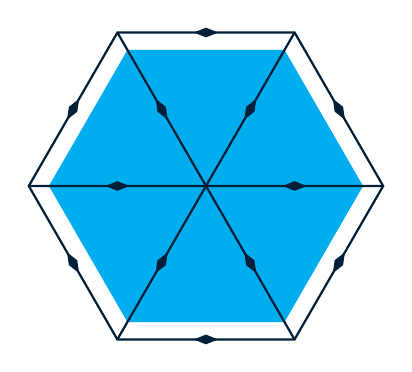
\begin{tikzpicture}[scale=1.5]
        \coordinate (0-0) at (1.5, 0);
        \coordinate (0-1) at (3, 0);
        \coordinate (1-0) at ($(0-0) + (120:1.5)$);
        \coordinate (1-1) at ($(1-0) + (1.5, 0)$);
        \coordinate (1-2) at ($(1-0) + (3, 0)$);
        \coordinate (2-0) at ($(1-0) + (60:1.5)$);
        \coordinate (2-1) at ($(2-0) + (1.5, 0)$);

        \draw[blue, line join=miter, thick] (0-0) -- (0-1) -- (1-2)
        -- (2-1) -- (2-0) -- (1-0) -- cycle;
        \draw[blue, line join=miter, thick] (0-0) -- (1-1) -- (2-1);
        \draw[blue, line join=miter, thick] (1-0) -- (1-1) -- (1-2);
        \draw[blue, line join=miter, thick] (2-0) -- (1-1) -- (0-1);

        \node[transform shape, shape=diamond, fill=blue,blue,
        inner sep=0pt, minimum height=2.5pt, minimum width=6pt] at
        ($(0-0)!0.5!(0-1)$) {};

        \node[transform shape, shape=diamond, fill=blue,blue,
        inner sep=0pt, minimum height=2.5pt, minimum width=6pt] at
        ($(1-0)!0.5!(1-1)$) {};

        \node[transform shape, shape=diamond, fill=blue,blue,
        inner sep=0pt, minimum height=2.5pt, minimum width=6pt] at
        ($(1-1)!0.5!(1-2)$) {};

        \node[transform shape, shape=diamond, fill=blue,blue,
        inner sep=0pt, minimum height=2.5pt, minimum width=6pt] at
        ($(2-0)!0.5!(2-1)$) {};

        \node[transform shape, shape=diamond, fill=blue,blue,
        inner sep=0pt, minimum height=2.5pt, minimum width=6pt, rotate=120] at
        ($(0-0)!0.5!(1-0)$) {};

        \node[transform shape, shape=diamond, fill=blue,blue,
        inner sep=0pt, minimum height=2.5pt, minimum width=6pt, rotate=120] at
        ($(0-1)!0.5!(1-1)$) {};

        \node[transform shape, shape=diamond, fill=blue,blue,
        inner sep=0pt, minimum height=2.5pt, minimum width=6pt, rotate=120] at
        ($(1-1)!0.5!(2-0)$) {};

        \node[transform shape, shape=diamond, fill=blue,blue,
        inner sep=0pt, minimum height=2.5pt, minimum width=6pt, rotate=120] at
        ($(1-2)!0.5!(2-1)$) {};


        \node[transform shape, shape=diamond, fill=blue,blue,
        inner sep=0pt, minimum height=2.5pt, minimum width=6pt, rotate=60] at
        ($(1-0)!0.5!(2-0)$) {};

        \node[transform shape, shape=diamond, fill=blue,blue,
        inner sep=0pt, minimum height=2.5pt, minimum width=6pt, rotate=60] at
        ($(0-0)!0.5!(1-1)$) {};

        \node[transform shape, shape=diamond, fill=blue,blue,
        inner sep=0pt, minimum height=2.5pt, minimum width=6pt, rotate=60] at
        ($(1-1)!0.5!(2-1)$) {};

        \node[transform shape, shape=diamond, fill=blue,blue,
        inner sep=0pt, minimum height=2.5pt, minimum width=6pt, rotate=60] at
        ($(0-1)!0.5!(1-2)$) {};

        \begin{scope}[on background layer]
          \draw[cyan, fill=cyan] ([shift={(60:5pt)}]0-0) --
          ([shift={(120:5pt)}]0-1) --
          ([shift={(180:5pt)}]1-2) --
          ([shift={(240:5pt)}]2-1) --
          ([shift={(300:5pt)}]2-0) --
          ([shift={(0:5pt)}]1-0) --
          cycle;
        \end{scope}
      \end{tikzpicture}
    \end{minipage}

    \vspace{1.75\baselineskip}
    {\centering\Large\bfseries H(div) multigrid\strut\par}
    \vspace{-0.75\baselineskip}
    \begin{equation*}
      (u, v) + \alpha(\nabla \cdot u, \nabla \cdot v) = (f, v)
    \end{equation*}
    \begin{minipage}[t]{0.66\linewidth}
\begin{minted}{text}
-mg_levels_pc_type patch
-mg_levels_pc_patch_construct_type star
-mg_levels_pc_patch_construct_dim 1
\end{minted}
      \begin{tabular}{cc|ccccc}
        \toprule
        levels & DoFs & \multicolumn{5}{c}{$\alpha$} \\
                  && $10^0$ & $10^1$ & $10^2$ & $10^3$ & $10^4$ \\
        \midrule
        1 & $1.26 \times 10^{4}$ & 40 & 42 & 43 & 44 & 44\\
        2 & $9.84 \times 10^{4}$ & 42 & 43 & 43 & 43 & 43\\
        3 & $7.78 \times 10^{5}$ & 45 & 45 & 45 & 45 & 45\\
        4 & $6.18 \times 10^{6}$ & 46 & 47 & 47 & 47 & 47\\
        \bottomrule
      \end{tabular}
    \end{minipage}
    \hfill
    \begin{minipage}[t]{0.33\linewidth}
      \strut\vspace*{-\baselineskip}\newline
      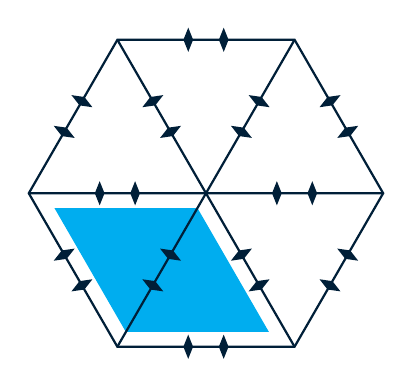
\begin{tikzpicture}[scale=1.5]
        \coordinate (0-0) at (1.5, 0);
        \coordinate (0-1) at (3, 0);
        \coordinate (1-0) at ($(0-0) + (120:1.5)$);
        \coordinate (1-1) at ($(1-0) + (1.5, 0)$);
        \coordinate (1-2) at ($(1-0) + (3, 0)$);
        \coordinate (2-0) at ($(1-0) + (60:1.5)$);
        \coordinate (2-1) at ($(2-0) + (1.5, 0)$);

        \draw[blue, line join=miter, thick] (0-0) -- (0-1) -- (1-2)
        -- (2-1) -- (2-0) -- (1-0) -- cycle;
        \draw[blue, line join=miter, thick] (0-0) -- (1-1) -- (2-1);
        \draw[blue, line join=miter, thick] (1-0) -- (1-1) -- (1-2);
        \draw[blue, line join=miter, thick] (2-0) -- (1-1) -- (0-1);

        \foreach \i in {0.4, 0.6} {
        \node[transform shape, shape=diamond, fill=blue,blue,
        inner sep=0pt, minimum height=6pt, minimum width=2.5pt] at
        ($(0-0)!\i!(0-1)$) {};

        \node[transform shape, shape=diamond, fill=blue,blue,
        inner sep=0pt, minimum height=6pt, minimum width=2.5pt] at
        ($(1-0)!\i!(1-1)$) {};

        \node[transform shape, shape=diamond, fill=blue,blue,
        inner sep=0pt, minimum height=6pt, minimum width=2.5pt] at
        ($(1-1)!\i!(1-2)$) {};

        \node[transform shape, shape=diamond, fill=blue,blue,
        inner sep=0pt, minimum height=6pt, minimum width=2.5pt] at
        ($(2-0)!\i!(2-1)$) {};

        \node[transform shape, shape=diamond, fill=blue,blue,
        inner sep=0pt, minimum height=6pt, minimum width=2.5pt, rotate=120] at
        ($(0-0)!\i!(1-0)$) {};

        \node[transform shape, shape=diamond, fill=blue,blue,
        inner sep=0pt, minimum height=6pt, minimum width=2.5pt, rotate=120] at
        ($(0-1)!\i!(1-1)$) {};

        \node[transform shape, shape=diamond, fill=blue,blue,
        inner sep=0pt, minimum height=6pt, minimum width=2.5pt, rotate=120] at
        ($(1-1)!\i!(2-0)$) {};

        \node[transform shape, shape=diamond, fill=blue,blue,
        inner sep=0pt, minimum height=6pt, minimum width=2.5pt, rotate=120] at
        ($(1-2)!\i!(2-1)$) {};


        \node[transform shape, shape=diamond, fill=blue,blue,
        inner sep=0pt, minimum height=6pt, minimum width=2.5pt, rotate=60] at
        ($(1-0)!\i!(2-0)$) {};

        \node[transform shape, shape=diamond, fill=blue,blue,
        inner sep=0pt, minimum height=6pt, minimum width=2.5pt, rotate=60] at
        ($(0-0)!\i!(1-1)$) {};

        \node[transform shape, shape=diamond, fill=blue,blue,
        inner sep=0pt, minimum height=6pt, minimum width=2.5pt, rotate=60] at
        ($(1-1)!\i!(2-1)$) {};

        \node[transform shape, shape=diamond, fill=blue,blue,
        inner sep=0pt, minimum height=6pt, minimum width=2.5pt, rotate=60] at
        ($(0-1)!\i!(1-2)$) {};
        }
        \begin{scope}[on background layer]
          \draw[cyan, fill=cyan] ($(0-0) + (60:0.15)$) --
          ($(0-0) + (60:0.15) + (0:1.2)$) --
          ($(1-1) + (240:0.15)$) --
          ($(1-1) + (240:0.15) + (180:1.2)$) -- 
          cycle;
        \end{scope}
      \end{tikzpicture}
    \end{minipage}

    \vspace{1.75\baselineskip}
    {\centering\Large\bfseries Nearly-incompressible elasticity\par}
    \vspace{-0.75\baselineskip}
    \begin{equation*}
      (\varepsilon(u),\varepsilon(v)) + \alpha(\nabla \cdot u, \nabla
      \cdot v) = (f, v)
    \end{equation*}
    \begin{minipage}[t]{0.66\linewidth}
\begin{minted}{python}
def macropatch(self, mesh, vertex):
  s = mesh.star(vertex)
  c = concat(*(mesh.closure(p) for p in s))
  return concat(s, *(mesh.star(p) for p in c))
\end{minted}
      \vspace{0pt}
\begin{minted}{text}
-mg_levels_pc_type patch
-mg_levels_pc_patch_construct_dim 0
-mg_levels_pc_patch_construct_type python
-mg_levels_pc_patch_construct_python_type macropatch
\end{minted}
      \begin{tabular}{cr|cccccccc}
        \toprule
        levels & DoFs               & \multicolumn{7}{c}{$\alpha$}                                 \\
                  &                    & $10^0$ & $10^1$ & $10^2$ & $10^3$ & $10^4$ & $10^6$ & $10^8$ \\
        \midrule
        1         & $2.39 \times 10^4$ & 15       & 14   & 18     & 23     & 25     & 26     & 25     \\
        2         & $1.85\times 10^5$  & 16       & 16   & 21     & 26     & 29     & 31     & 30     \\
        3         & $1.46\times 10^6$  & 16       & 16   & 22     & 27     & 31     & 32     & 31     \\
        \bottomrule
      \end{tabular}
    \end{minipage}
    \hfill
    \begin{minipage}[t]{0.33\linewidth}
      \strut\vspace*{-\baselineskip}\newline
      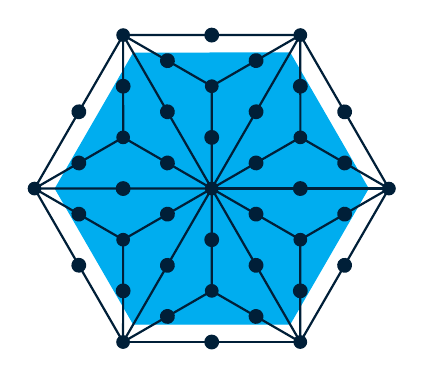
\begin{tikzpicture}[scale=1.5,
        dof/.style={blue, postaction={decorate,decoration={markings,
              mark=at position 0.5 with {\draw[solid, fill=blue, blue] circle (0.08);}}}
        }]
        \coordinate (0-0) at (1.5, 0);
        \coordinate (0-1) at (3, 0);
        \coordinate (1-0) at ($(0-0) + (120:1.5)$);
        \coordinate (1-1) at ($(1-0) + (1.5, 0)$);
        \coordinate (1-2) at ($(1-0) + (3, 0)$);
        \coordinate (2-0) at ($(1-0) + (60:1.5)$);
        \coordinate (2-1) at ($(2-0) + (1.5, 0)$);
        \foreach \i in {0, 1, 2} {
          \foreach \j in {0, 1} {
            \draw[fill=blue, blue] (\i-\j) circle (0.053333);
          }
        }
        \draw[fill=blue, blue] (1-2) circle (0.053333);

        \coordinate (bc0) at (barycentric cs:0-0=1,1-0=1,1-1=1);
        \coordinate (bc1) at (barycentric cs:0-0=1,0-1=1,1-1=1);
        \coordinate (bc2) at (barycentric cs:0-1=1,1-1=1,1-2=1);
        \coordinate (bc3) at (barycentric cs:1-0=1,1-1=1,2-0=1);
        \coordinate (bc4) at (barycentric cs:1-1=1,2-0=1,2-1=1);
        \coordinate (bc5) at (barycentric cs:1-1=1,2-1=1,1-2=1);
        \foreach \i in {0, 1, 2, 3, 4, 5} {
          \draw[fill=blue, blue] (bc\i) circle (0.053333);
        }

        \draw[dof, line join=miter, thick] (0-0) -- (0-1);
        \draw[dof, line join=miter, thick] (0-1) -- (1-2);
        \draw[dof, line join=miter, thick] (1-2) -- (2-1);
        \draw[dof, line join=miter, thick] (2-1) -- (2-0);
        \draw[dof, line join=miter, thick] (2-0) -- (1-0);
        \draw[dof, line join=miter, thick] (1-0) -- (0-0);

        \draw[dof, line join=miter, thick] (0-0) -- (1-1);
        \draw[dof, line join=miter, thick] (0-1) -- (1-1);
        \draw[dof, line join=miter, thick] (1-0) -- (1-1);
        \draw[dof, line join=miter, thick] (1-2) -- (1-1);
        \draw[dof, line join=miter, thick] (2-0) -- (1-1);
        \draw[dof, line join=miter, thick] (2-1) -- (1-1);

        \draw[dof, line join=miter, thick] (0-0) -- (bc0);
        \draw[dof, line join=miter, thick] (1-0) -- (bc0);
        \draw[dof, line join=miter, thick] (1-1) -- (bc0);

        \draw[dof, line join=miter, thick] (0-0) -- (bc1);
        \draw[dof, line join=miter, thick] (0-1) -- (bc1);
        \draw[dof, line join=miter, thick] (1-1) -- (bc1);

        \draw[dof, line join=miter, thick] (0-1) -- (bc2);
        \draw[dof, line join=miter, thick] (1-2) -- (bc2);
        \draw[dof, line join=miter, thick] (1-1) -- (bc2);

        \draw[dof, line join=miter, thick] (2-0) -- (bc3);
        \draw[dof, line join=miter, thick] (1-0) -- (bc3);
        \draw[dof, line join=miter, thick] (1-1) -- (bc3);

        \draw[dof, line join=miter, thick] (2-1) -- (bc4);
        \draw[dof, line join=miter, thick] (2-0) -- (bc4);
        \draw[dof, line join=miter, thick] (1-1) -- (bc4);

        \draw[dof, line join=miter, thick] (1-2) -- (bc5);
        \draw[dof, line join=miter, thick] (2-1) -- (bc5);
        \draw[dof, line join=miter, thick] (1-1) -- (bc5);
        \begin{scope}[on background layer]
          \draw[cyan, fill=cyan] ([shift={(60:5pt)}]0-0) --
          ([shift={(120:5pt)}]0-1) --
          ([shift={(180:5pt)}]1-2) --
          ([shift={(240:5pt)}]2-1) --
          ([shift={(300:5pt)}]2-0) --
          ([shift={(0:5pt)}]1-0) --
          cycle;
        \end{scope}
      \end{tikzpicture}
    \end{minipage}
  \end{posterbox}

  \begin{posterbox}[name=config, span=2,column=2, height=1]{Building blocks}
    \tcbset{center title,
      colframe=red,
      colback=red!10!white,
      colupper=blue,
      collower=blue,
      fonttitle=\bfseries,
      right=1mm,
      left=1mm,
      top=1mm,
      bottom=0.25mm,
      boxsep=0.5mm,
      middle=0mm,
      toptitle=-0.5mm,
      bottomtitle=-1mm,
      valign upper=top,
      valign lower=center,
      halign=left,
      lower separated=false,
      before title=\strut}
    \begin{tcolorbox}[title={Overview}]
      {\raggedright \texttt{PCPATCH} is a PETSc preconditioner
        providing configurable multigrid relaxation schemes based on
        topological space decompositions. Out of the box, it offers
        runtime access to overlapping block smoothers for many nearly
        singular problems, as well as Vanka-like relaxation for
        all-at-once multigrid.\par}
    \end{tcolorbox}
    \begin{tcolorbox}[title={Topological queries}]
      Dimension and cell-shape independent specification of
      decompositions via \texttt{DMPlex}.

      \vspace{0.5\baselineskip}

      \begin{minipage}[c]{0.32\textwidth}
        {\centering 
          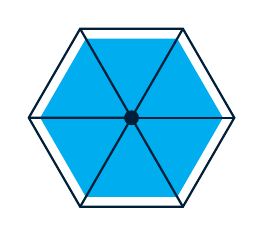
\begin{tikzpicture}[scale=0.87]
            \coordinate (0-0) at (1.5, 0); \coordinate (0-1) at (3,
            0); \coordinate (1-0) at ($(0-0) + (120:1.5)$);
            \coordinate (1-1) at ($(1-0) + (1.5, 0)$); \coordinate
            (1-2) at ($(1-0) + (3, 0)$); \coordinate (2-0) at
            ($(1-0) + (60:1.5)$); \coordinate (2-1) at
            ($(2-0) + (1.5, 0)$);

            \draw[blue, line join=miter, thick] (0-0) -- (0-1) --
            (1-2) -- (2-1) -- (2-0) -- (1-0) -- cycle;
            \draw[blue, line join=miter, thick] (0-0) -- (1-1);
            \draw[blue, line join=miter, thick] (0-1) -- (1-1);
            \draw[blue, line join=miter, thick] (1-0) -- (1-1);
            \draw[blue, line join=miter, thick] (1-2) -- (1-1);
            \draw[blue, line join=miter, thick] (2-0) -- (1-1);
            \draw[blue, line join=miter, thick] (2-1) -- (1-1);
            \draw[solid, blue, fill=blue] (1-1) circle (0.1);
            \begin{scope}[on background layer]
              \draw[cyan, fill=cyan] ([shift={(60:5pt)}]0-0) --
              ([shift={(120:5pt)}]0-1) -- ([shift={(180:5pt)}]1-2) --
              ([shift={(240:5pt)}]2-1) -- ([shift={(300:5pt)}]2-0) --
              ([shift={(0:5pt)}]1-0) -- cycle;
            \end{scope}
          \end{tikzpicture}

          \texttt{star(vertex)\strut}
          \par
        }
      \end{minipage}
      \hfill
      \begin{minipage}[c]{0.32\textwidth}
        {\centering
          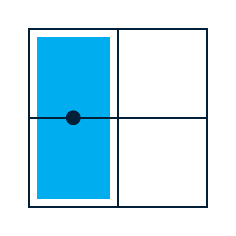
\begin{tikzpicture}[scale=0.87]
            \coordinate (0-0) at (0, 0);
            \coordinate (0-1) at ($({sin(60) * 1.5}, 0)$);
            \coordinate (0-2) at ($({sin(60) * 3}, 0)$);
            \coordinate (1-0) at ($({sin(60) * 0}, {sin(60) * 1.5})$);
            \coordinate (1-1) at ($({sin(60) * 1.5}, {sin(60) * 1.5})$);
            \coordinate (1-2) at ($({sin(60) * 3}, {sin(60) * 1.5})$);
            \coordinate (2-0) at ($({sin(60) * 0}, {sin(60) * 3})$);
            \coordinate (2-1) at ($({sin(60) * 1.5}, {sin(60) * 3})$);
            \coordinate (2-2) at ($({sin(60) * 3}, {sin(60) * 3})$);

            \draw[blue, line join=miter, thick] (0-0) -- (0-1) --
            (0-2) -- (1-2) -- (2-2) -- (2-1) -- (2-0) -- (1-0) -- cycle;
            \draw[blue, line join=miter, thick] (1-0) -- (1-1) -- (1-2);
            \draw[blue, line join=miter, thick] (0-1) -- (1-1) -- (2-1);

            \draw[solid, blue, fill=blue] ($(1-0)!0.5!(1-1)$) circle
            (0.1);
            \begin{scope}[on background layer]
              \draw[cyan, fill=cyan] ([shift={(45:5pt)}]0-0) --
              ([shift={(135:5pt)}]0-1) -- ([shift={(225:5pt)}]2-1) --
              ([shift={(315:5pt)}]2-0) -- cycle;
            \end{scope}
          \end{tikzpicture}

          \texttt{star(edge)\strut}
          \par
        }
      \end{minipage}
      \hfill
      \begin{minipage}[c]{0.32\textwidth}
        {\raggedright \texttt{star} relation gathers incident entities with equal or
          smaller codimension.\par}
      \end{minipage}

      \vspace{1\baselineskip}

      \begin{minipage}[c]{0.32\textwidth}
        {\raggedright \texttt{closure} relation gathers incident entities with equal or
          smaller dimension.\par}
      \end{minipage}
      \hfill
      \begin{minipage}[c]{0.32\textwidth}
        {\centering
          
\begin{tikzpicture}[scale=0.79]
            \coordinate (0-0) at (1.5, 0); \coordinate (0-1) at (3,
            0); \coordinate (1-0) at ($(0-0) + (120:1.5)$);
            \coordinate (1-1) at ($(1-0) + (1.5, 0)$); \coordinate
            (1-2) at ($(1-0) + (3, 0)$); \coordinate (2-0) at
            ($(1-0) + (60:1.5)$); \coordinate (2-1) at
            ($(2-0) + (1.5, 0)$);
            \draw[blue, line join=miter, thick] (0-0) -- (0-1) --
            (1-2) -- (2-1) -- (2-0) -- (1-0) -- cycle;
            \draw[blue, line join=miter, thick] (0-0) -- (1-1);
            \draw[blue, line join=miter, thick] (0-1) -- (1-1);
            \draw[blue, line join=miter, thick] (1-0) -- (1-1);
            \draw[blue, line join=miter, thick] (1-2) -- (1-1);
            \draw[blue, line join=miter, thick] (2-0) -- (1-1);
            \draw[blue, line join=miter, thick] (2-1) -- (1-1);
            \draw[solid, blue, fill=blue] (barycentric cs:1-1=1,1-0=1,0-0=1) circle (0.1);
            \begin{scope}[on background layer]
              \draw[cyan, fill=cyan] ([shift={(270:7.5pt)}]0-0) --
              ([shift={(30:7.5pt)}]1-1) --
              ([shift={(150:7.5pt)}]1-0) --
              cycle;
            \end{scope}
          \end{tikzpicture}

          \texttt{closure(cell)\strut}
          \par
        }
      \end{minipage}
      \hfill
      \begin{minipage}[c]{0.32\textwidth}
        {\centering
          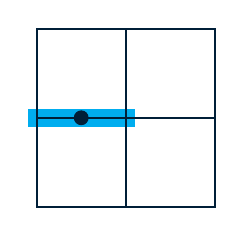
\begin{tikzpicture}[scale=0.87]
            \coordinate (0-0) at (0, 0);
            \coordinate (0-1) at ($({sin(60) * 1.5}, 0)$);
            \coordinate (0-2) at ($({sin(60) * 3}, 0)$);
            \coordinate (1-0) at ($({sin(60) * 0}, {sin(60) * 1.5})$);
            \coordinate (1-1) at ($({sin(60) * 1.5}, {sin(60) * 1.5})$);
            \coordinate (1-2) at ($({sin(60) * 3}, {sin(60) * 1.5})$);
            \coordinate (2-0) at ($({sin(60) * 0}, {sin(60) * 3})$);
            \coordinate (2-1) at ($({sin(60) * 1.5}, {sin(60) * 3})$);
            \coordinate (2-2) at ($({sin(60) * 3}, {sin(60) * 3})$);

            \draw[blue, line join=miter, thick] (0-0) -- (0-1) --
            (0-2) -- (1-2) -- (2-2) -- (2-1) -- (2-0) -- (1-0) -- cycle;
            \draw[blue, line join=miter, thick] (1-0) -- (1-1) -- (1-2);
            \draw[blue, line join=miter, thick] (0-1) -- (1-1) -- (2-1);

            \draw[solid, blue, fill=blue] ($(1-0)!0.5!(1-1)$) circle
            (0.1);
            \begin{scope}[on background layer]
              \draw[cyan, fill=cyan]
              ([shift={(45:5pt)}]1-1) -- ([shift={(135:5pt)}]1-0) --
              ([shift={(225:5pt)}]1-0) -- ([shift={(315:5pt)}]1-1) -- cycle;
            \end{scope}
          \end{tikzpicture}

          \texttt{closure(edge)\strut}
          \par
        }
      \end{minipage}
    \end{tcolorbox}

    \begin{tcolorbox}[title={Jacobian and residual evaluation},
      halign=left]
      \begin{minipage}[t]{0.75\linewidth}
        {\raggedright \texttt{PCPATCH} constructs local DoF numberings for each
          patch and coordinates iteration over patches. Callback
          interface to discretisation engine for Jacobian and residual
          evaluation enables nonlinear and matrix-free relaxation.\par}
\begin{minted}{c}
int Jacobian(PC pc, PetscInt point, Vec state, 
  Mat J, IS entities, PetscInt ndof, 
  PetscInt *dofNumbering, void *ctx);
int Residual(PC pc, PetscInt point, Vec state, 
  Vec F, IS entities, PetscInt ndof, 
  PetscInt *dofNumbering, void *ctx);
\end{minted}
      \end{minipage}
      \hfill
      \begin{minipage}[t]{0.24\linewidth}
        \strut\vspace*{-\baselineskip}\newline
        {\centering
          
\includegraphics[width=0.5\textwidth]{firedrake-noword}
          \par
        }
        \vspace{0.5\baselineskip}
        {\centering
          \texttt{DMPlex + PetscDS}
          \vspace{0.5\baselineskip}

          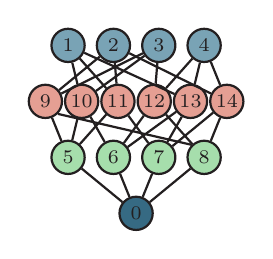
\begin{tikzpicture}[scale=0.9]
            \tikzstyle{line} = [draw, -, thick]
            \tikzstyle{nodraw} = [draw, fill, circle, minimum width=0pt, inner sep=0pt]
            \tikzstyle{sieve} = [line, circle, font=\scriptsize, inner sep=0pt, minimum size=12pt]
            \tikzstyle{cell} = [sieve, fill=blue!60]
            \tikzstyle{facet} = [sieve, fill=green!35]
            \tikzstyle{edge} = [sieve, fill=red!35]
            \tikzstyle{vertex} = [sieve, fill=blue!35]
            \def\y{.79}
\def\x{.32}
\node (0) [cell] at (0,0) {0};
\node (1) [facet] at (-3*\x, \y) {5};
\node (2) [facet] at (-1*\x, \y) {6};
\node (3) [facet] at (1*\x, \y) {7};
\node (4) [facet] at (3*\x, \y) {8};
\node (5) [edge] at (-4*\x, 2*\y) {9};
\node (6) [edge] at (-2.4*\x, 2*\y) {10};
\node (7) [edge] at (-.8*\x, 2*\y) {11};
\node (8) [edge] at (.8*\x, 2*\y) {12};
\node (9) [edge] at (2.4*\x, 2*\y) {13};
\node (10) [edge] at (4*\x, 2*\y) {14};
\node (11) [vertex] at (-3*\x, 3*\y) {1};
\node (12) [vertex] at (-1*\x, 3*\y) {2};
\node (13) [vertex] at (1*\x, 3*\y) {3};
\node (14) [vertex] at (3*\x, 3*\y) {4};

\draw[line] (0) -- (1);
\draw[line] (0) -- (2);
\draw[line] (0) -- (3);
\draw[line] (0) -- (4);
\draw[line] (1) -- (5);
\draw[line] (1) -- (6);
\draw[line] (1) -- (7);
\draw[line] (2) -- (6);
\draw[line] (2) -- (8);
\draw[line] (2) -- (9);
\draw[line] (3) -- (7);
\draw[line] (3) -- (9);
\draw[line] (3) -- (10);
\draw[line] (4.north west) -- (5.south east);
\draw[line] (4) -- (8);
\draw[line] (4) -- (10);
\draw[line] (5) -- (12);
\draw[line] (5) -- (13);
\draw[line] (6) -- (11);
\draw[line] (6) -- (13);
\draw[line] (7) -- (11);
\draw[line] (7) -- (12);
\draw[line] (8) -- (13);
\draw[line] (8) -- (14);
\draw[line] (9) -- (11);
\draw[line] (9) -- (14);
\draw[line] (10) -- (12);
\draw[line] (10) -- (14);

          \end{tikzpicture}
          \par
        }
      \end{minipage}
    \end{tcolorbox}
    \begin{tcolorbox}[title={Relaxation schemes}]
      \begin{algorithm}[H]
        \SetKwInOut{Input}{input}
        \SetKwInOut{Output}{output}
        \Input{\,Initial guess $u^k \in V$, weighting operators $w_i : V_i \to V_i$}
        \Output{\,Updated guess $u^{k+1} \in V$}
        \BlankLine
        \For{$i = 1$ \KwTo $J$}{ Find
          $\delta u_i \in V_i$ such that
          \begin{equation*}
            \begin{aligned}
              a(\delta u_i, v_i)       & = (f, v_i) - a(u^k, v_i) && \text{linear case}       & \text{\texttt{-pc\_type patch}} \\
              F(u^k + \delta u_i; v_i) & = 0                      && \text{nonlinear case} & \text{\texttt{-snes\_type patch}}
            \end{aligned}
          \end{equation*}
        } $u^{k+1} \gets u^k + \sum_{i=1}^{J} w_i(\delta u_i)$
      \end{algorithm}
    \end{tcolorbox}
  \end{posterbox}
  \begin{posterbox}[name=examples, column=4, span=2, height=0.85]{Examples}
    \vspace{0.25\baselineskip}
    {\centering\Large\bfseries Vanka relaxation for Stokes\strut\par}

    Find $(u, p) \in V\times Q := \mathbb{P}_2^2 \times \mathbb{P}_1$ such that
    \vspace{-0.75\baselineskip}
    \begin{equation*}
      \nu (\varepsilon{(u)}, \varepsilon{(v)}) - (p, \nabla \cdot v) -
      (\nabla \cdot u, q) = (f, v) \quad \forall (v, q) \in V \times Q.
    \end{equation*}

    \begin{minipage}[t]{0.49\linewidth}
      \strut\vspace*{-\baselineskip}\newline
      {\centering
        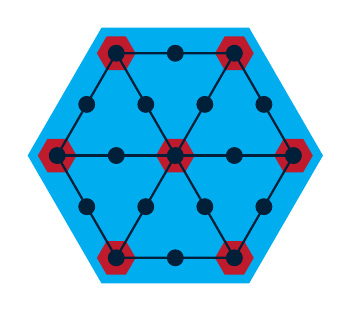
\begin{tikzpicture}
          \coordinate (0-0) at (1.5, 0);
          \coordinate (0-1) at (3, 0);
          \coordinate (1-0) at ($(0-0) + (120:1.5)$);
          \coordinate (1-1) at ($(1-0) + (1.5, 0)$);
          \coordinate (1-2) at ($(1-0) + (3, 0)$);
          \coordinate (2-0) at ($(1-0) + (60:1.5)$);
          \coordinate (2-1) at ($(2-0) + (1.5, 0)$);
          \draw[blue, line join=miter, thick] (0-0) -- (0-1) -- (1-2)
          -- (2-1) -- (2-0) -- (1-0) -- cycle;
          \draw[blue, line join=miter, thick] (0-0) -- (1-1) -- (2-1);
          \draw[blue, line join=miter, thick] (1-0) -- (1-1) -- (1-2);
          \draw[blue, line join=miter, thick] (2-0) -- (1-1) -- (0-1);

          \begin{scope}[on background layer]
            \node[regular polygon, regular polygon sides=6, transform
            shape, fill=cyan, cyan, inner sep=0pt, minimum height=3.75cm, minimum width=3.75cm] at (1-1) {};
          \end{scope}
          \begin{scope}[on background layer]
            \node[regular polygon, regular polygon sides=6, transform shape, fill=red, red, inner sep=0pt, minimum height=14pt, minimum width=14pt] at (0-0) {};
            \node[regular polygon, regular polygon sides=6, transform shape, fill=red, red, inner sep=0pt, minimum height=14pt, minimum width=14pt] at (0-1) {};
            \node[regular polygon, regular polygon sides=6, transform shape, fill=red, red, inner sep=0pt, minimum height=14pt, minimum width=14pt] at (1-0) {};
            \node[regular polygon, regular polygon sides=6, transform shape, fill=red, red, inner sep=0pt, minimum height=14pt, minimum width=14pt] at (1-1) {};
            \node[regular polygon, regular polygon sides=6, transform shape, fill=red, red, inner sep=0pt, minimum height=14pt, minimum width=14pt] at (1-2) {};
            \node[regular polygon, regular polygon sides=6, transform shape, fill=red, red, inner sep=0pt, minimum height=14pt, minimum width=14pt] at (2-0) {};
            \node[regular polygon, regular polygon sides=6, transform shape, fill=red, red, inner sep=0pt, minimum height=14pt, minimum width=14pt] at (2-1) {};
            
          \end{scope}
          \draw[solid, blue, fill=blue] (0-0) circle (0.1);
          \draw[solid, blue, fill=blue] (0-1) circle (0.1);
          \draw[solid, blue, fill=blue] (1-0) circle (0.1);
          \draw[solid, blue, fill=blue] (1-1) circle (0.1);
          \draw[solid, blue, fill=blue] (1-2) circle (0.1);
          \draw[solid, blue, fill=blue] (2-0) circle (0.1);
          \draw[solid, blue, fill=blue] (2-1) circle (0.1);

          \draw[solid, blue, fill=blue] ($(0-0)!0.5!(0-1)$) circle (0.1);
          \draw[solid, blue, fill=blue] ($(0-1)!0.5!(1-2)$) circle (0.1);
          \draw[solid, blue, fill=blue] ($(1-2)!0.5!(2-1)$) circle (0.1);
          \draw[solid, blue, fill=blue] ($(2-0)!0.5!(2-1)$) circle (0.1);
          \draw[solid, blue, fill=blue] ($(2-0)!0.5!(1-0)$) circle (0.1);
          \draw[solid, blue, fill=blue] ($(1-0)!0.5!(0-0)$) circle (0.1);

          \draw[solid, blue, fill=blue] ($(0-0)!0.5!(1-1)$) circle (0.1);
          \draw[solid, blue, fill=blue] ($(0-1)!0.5!(1-1)$) circle (0.1);
          \draw[solid, blue, fill=blue] ($(1-0)!0.5!(1-1)$) circle (0.1);
          \draw[solid, blue, fill=blue] ($(1-2)!0.5!(1-1)$) circle (0.1);
          \draw[solid, blue, fill=blue] ($(2-0)!0.5!(1-1)$) circle (0.1);
          \draw[solid, blue, fill=blue] ($(2-1)!0.5!(1-1)$) circle (0.1);
        \end{tikzpicture}
        \par
      }

\begin{minted}{text}
-pc_patch_construct_dim 0
-pc_patch_construct_type vanka
-pc_patch_exclude_subspaces 1

\end{minted}
    \end{minipage}
    \hfill
    \begin{minipage}[t]{0.49\linewidth}
      \strut\vspace*{-\baselineskip}\newline
      {\centering
        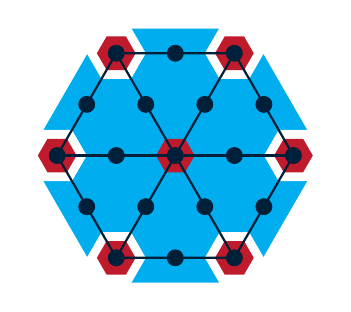
\begin{tikzpicture}
          \coordinate (0-0) at (1.5, 0);
          \coordinate (0-1) at (3, 0);
          \coordinate (1-0) at ($(0-0) + (120:1.5)$);
          \coordinate (1-1) at ($(1-0) + (1.5, 0)$);
          \coordinate (1-2) at ($(1-0) + (3, 0)$);
          \coordinate (2-0) at ($(1-0) + (60:1.5)$);
          \coordinate (2-1) at ($(2-0) + (1.5, 0)$);
          \draw[blue, line join=miter, thick] (0-0) -- (0-1) -- (1-2)
          -- (2-1) -- (2-0) -- (1-0) -- cycle;
          \draw[blue, line join=miter, thick] (0-0) -- (1-1) -- (2-1);
          \draw[blue, line join=miter, thick] (1-0) -- (1-1) -- (1-2);
          \draw[blue, line join=miter, thick] (2-0) -- (1-1) -- (0-1);

          \begin{scope}[on background layer]
            \node[regular polygon, regular polygon sides=6, transform
            shape, fill=cyan, cyan, inner sep=0pt, minimum
            height=3.725cm, minimum width=3.725cm] at (1-1) {};

            \node[regular polygon, regular polygon sides=6, transform shape, fill=white, white, inner sep=0pt, minimum height=0.75cm, minimum width=0.75cm] at (0-0) {};
            \node[regular polygon, regular polygon sides=6, transform shape, fill=white, white, inner sep=0pt, minimum height=0.75cm, minimum width=0.75cm] at (0-1) {};
            \node[regular polygon, regular polygon sides=6, transform shape, fill=white, white, inner sep=0pt, minimum height=0.75cm, minimum width=0.75cm] at (1-0) {};
            \node[regular polygon, regular polygon sides=6, transform shape, fill=white, white, inner sep=0pt, minimum height=0.75cm, minimum width=0.75cm] at (1-2) {};
            \node[regular polygon, regular polygon sides=6, transform shape, fill=white, white, inner sep=0pt, minimum height=0.75cm, minimum width=0.75cm] at (2-0) {};
            \node[regular polygon, regular polygon sides=6, transform shape, fill=white, white, inner sep=0pt, minimum height=0.75cm, minimum width=0.75cm] at (2-1) {};
          \end{scope}
          \begin{scope}[on background layer]
            \node[regular polygon, regular polygon sides=6, transform shape, fill=red, red, inner sep=0pt, minimum height=14pt, minimum width=14pt] at (0-0) {};
            \node[regular polygon, regular polygon sides=6, transform shape, fill=red, red, inner sep=0pt, minimum height=14pt, minimum width=14pt] at (0-1) {};
            \node[regular polygon, regular polygon sides=6, transform shape, fill=red, red, inner sep=0pt, minimum height=14pt, minimum width=14pt] at (1-0) {};
            \node[regular polygon, regular polygon sides=6, transform shape, fill=red, red, inner sep=0pt, minimum height=14pt, minimum width=14pt] at (1-1) {};
            \node[regular polygon, regular polygon sides=6, transform shape, fill=red, red, inner sep=0pt, minimum height=14pt, minimum width=14pt] at (1-2) {};
            \node[regular polygon, regular polygon sides=6, transform shape, fill=red, red, inner sep=0pt, minimum height=14pt, minimum width=14pt] at (2-0) {};
            \node[regular polygon, regular polygon sides=6, transform shape, fill=red, red, inner sep=0pt, minimum height=14pt, minimum width=14pt] at (2-1) {};
            
          \end{scope}
          \draw[solid, blue, fill=blue] (0-0) circle (0.1);
          \draw[solid, blue, fill=blue] (0-1) circle (0.1);
          \draw[solid, blue, fill=blue] (1-0) circle (0.1);
          \draw[solid, blue, fill=blue] (1-1) circle (0.1);
          \draw[solid, blue, fill=blue] (1-2) circle (0.1);
          \draw[solid, blue, fill=blue] (2-0) circle (0.1);
          \draw[solid, blue, fill=blue] (2-1) circle (0.1);

          \draw[solid, blue, fill=blue] ($(0-0)!0.5!(0-1)$) circle (0.1);
          \draw[solid, blue, fill=blue] ($(0-1)!0.5!(1-2)$) circle (0.1);
          \draw[solid, blue, fill=blue] ($(1-2)!0.5!(2-1)$) circle (0.1);
          \draw[solid, blue, fill=blue] ($(2-0)!0.5!(2-1)$) circle (0.1);
          \draw[solid, blue, fill=blue] ($(2-0)!0.5!(1-0)$) circle (0.1);
          \draw[solid, blue, fill=blue] ($(1-0)!0.5!(0-0)$) circle (0.1);

          \draw[solid, blue, fill=blue] ($(0-0)!0.5!(1-1)$) circle (0.1);
          \draw[solid, blue, fill=blue] ($(0-1)!0.5!(1-1)$) circle (0.1);
          \draw[solid, blue, fill=blue] ($(1-0)!0.5!(1-1)$) circle (0.1);
          \draw[solid, blue, fill=blue] ($(1-2)!0.5!(1-1)$) circle (0.1);
          \draw[solid, blue, fill=blue] ($(2-0)!0.5!(1-1)$) circle (0.1);
          \draw[solid, blue, fill=blue] ($(2-1)!0.5!(1-1)$) circle (0.1);
        \end{tikzpicture}
        \par
      }
\begin{minted}{text}
-pc_patch_construct_dim 0
-pc_patch_construct_type vanka
-pc_patch_exclude_subspaces 1
-pc_patch_vanka_dim 0
\end{minted}
    \end{minipage}

    \vspace{0.5\baselineskip}
    {\raggedleft\small Analysis of different patches in \texttt{arXiv:
        1908.09949 [math.NA]}\par}

    \vspace{0.5\baselineskip}
    \begin{minipage}[c]{0.4\textwidth}
      \strut\vspace*{-\baselineskip}\newline
      {\centering 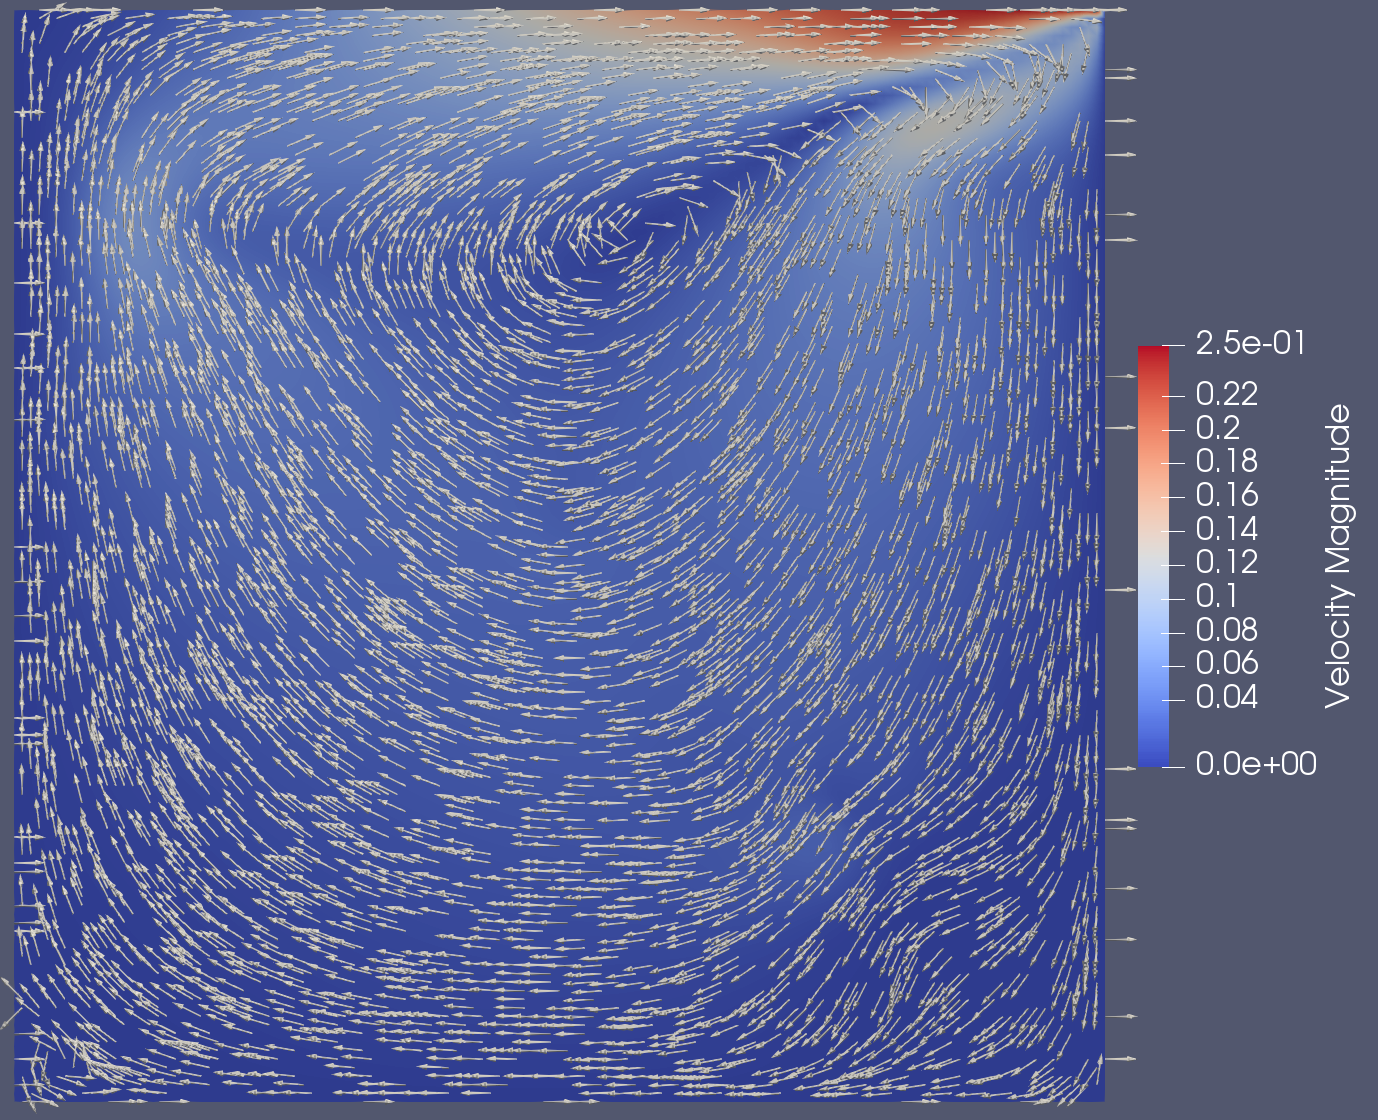
\includegraphics[height=2.25cm]{stokes-velocity}
        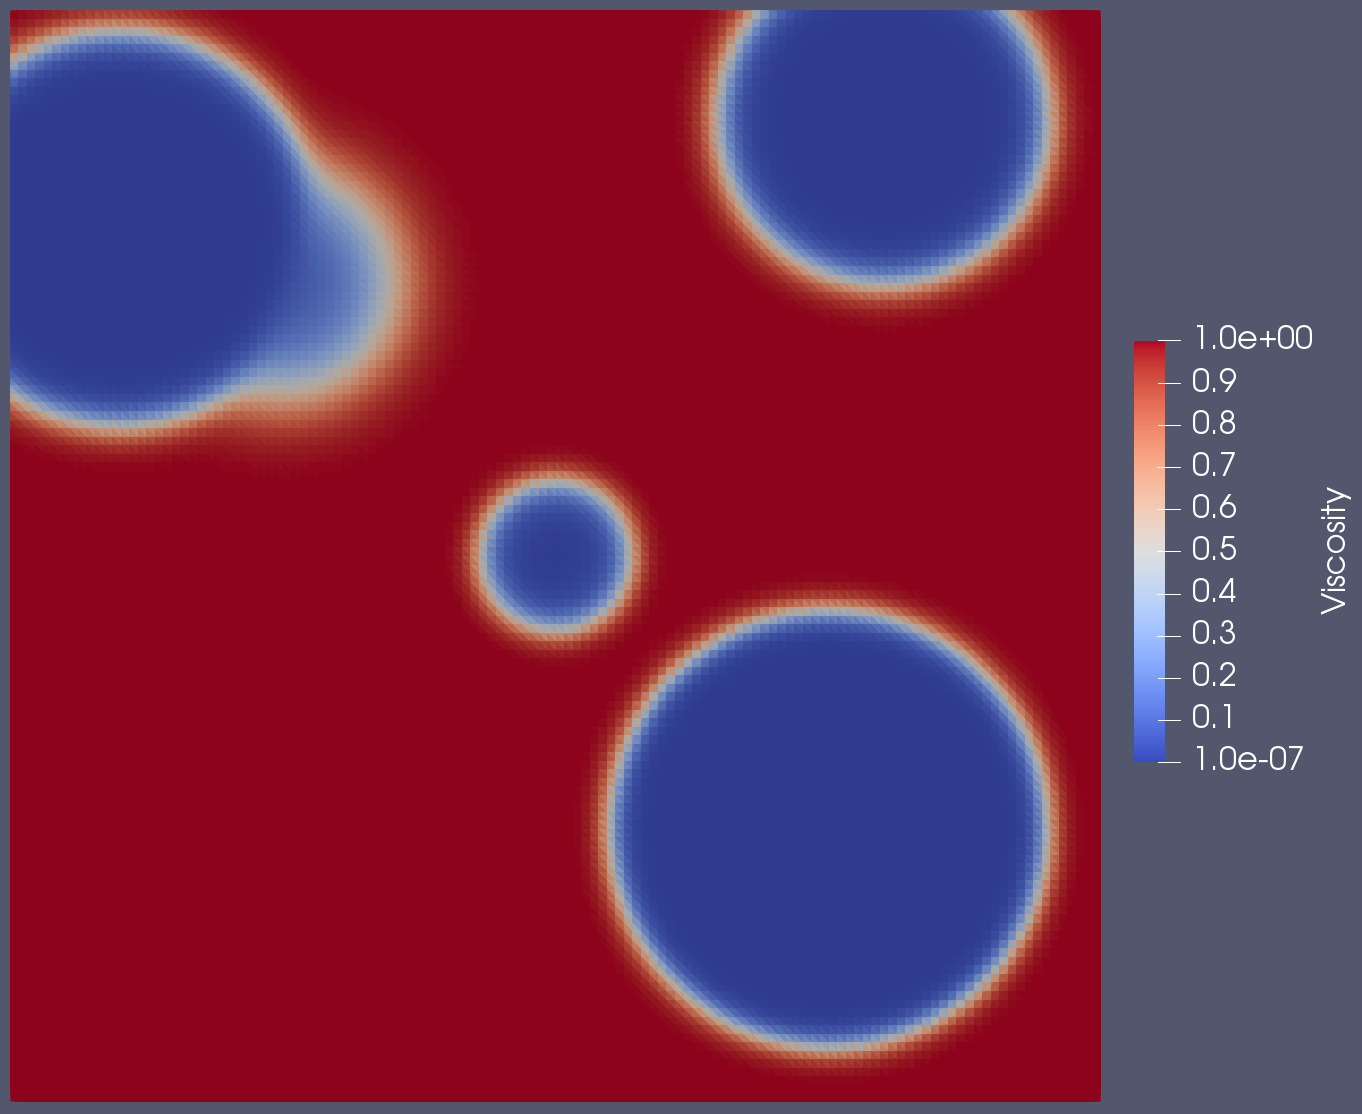
\includegraphics[height=2.25cm]{stokes-viscosity}\par}
    \end{minipage}
    \hfill
    \hspace{0.5em}
    \begin{minipage}[c]{0.6\textwidth}
      \strut\vspace*{-\baselineskip}\newline
      \begin{tabular}{cc|ccccc}
        \toprule
        levels & DoFs & \multicolumn{5}{c}{$\nu$} \\
                  && $10^0$ & $10^1$ & $10^2$ & $10^3$ & $10^4$ \\
        \midrule
        1 & $1.48 \times 10^{4}$ & 14 & 14 & 14 & 14 & 14\\
        2 & $5.84 \times 10^{4}$ & 14 & 14 & 14 & 14 & 14\\
        3 & $2.32 \times 10^{5}$ & 14 & 14 & 14 & 14 & 14\\
        4 & $9.25 \times 10^{5}$ & 14 & 14 & 14 & 14 & 14\\
        \bottomrule
      \end{tabular}
    \end{minipage}

    \vspace{1.75\baselineskip}
    {\centering\Large\bfseries Augmented Lagrangian preconditioning for
      Navier--Stokes\strut\par}
    \vspace{-0.75\baselineskip}
    \begin{equation*}
      \nu (\varepsilon{(u)}, \varepsilon{(v)}) + ((w \cdot \nabla) u,
      v) + ((u \cdot \nabla)w, v) + \gamma(\nabla \cdot u, \nabla \cdot v) = (f, v)
    \end{equation*}

    {\raggedright \texttt{PCPATCH} used to implement parameter-robust multigrid scheme
    for augmented Lagrangian momentum equation.\par}

    \begin{minipage}[c]{0.6\textwidth}
      \strut\vspace*{-\baselineskip}\newline
      \begin{tabular}{cc|ccccc}
        \toprule
        levels & DoFs & \multicolumn{5}{c}{Reynolds number} \\
               && 10 & 100 & 1000 & 2500 & 5000 \\
        \midrule
        1 & $2.1 \times 10^6$ & 4.50 & 4.00 & 5.00 & 4.50 & 4.00 \\
        2 & $1.7 \times 10^7$ & 4.50 & 4.33 & 4.50 & 4.00 & 4.00 \\
        3 & $1.3 \times 10^8$ & 4.50 & 4.33 & 4.00 & 3.50 & 7.00 \\
        4 & $1.1 \times 10^9$ & 4.50 & 3.66 & 3.00 & 5.00 & 5.00 \\
        \bottomrule
      \end{tabular}
    \end{minipage}
    \hfill
    \hspace{0.5em}
    \begin{minipage}[c]{0.4\textwidth}
      \strut\vspace*{-\baselineskip}\newline
      {\centering 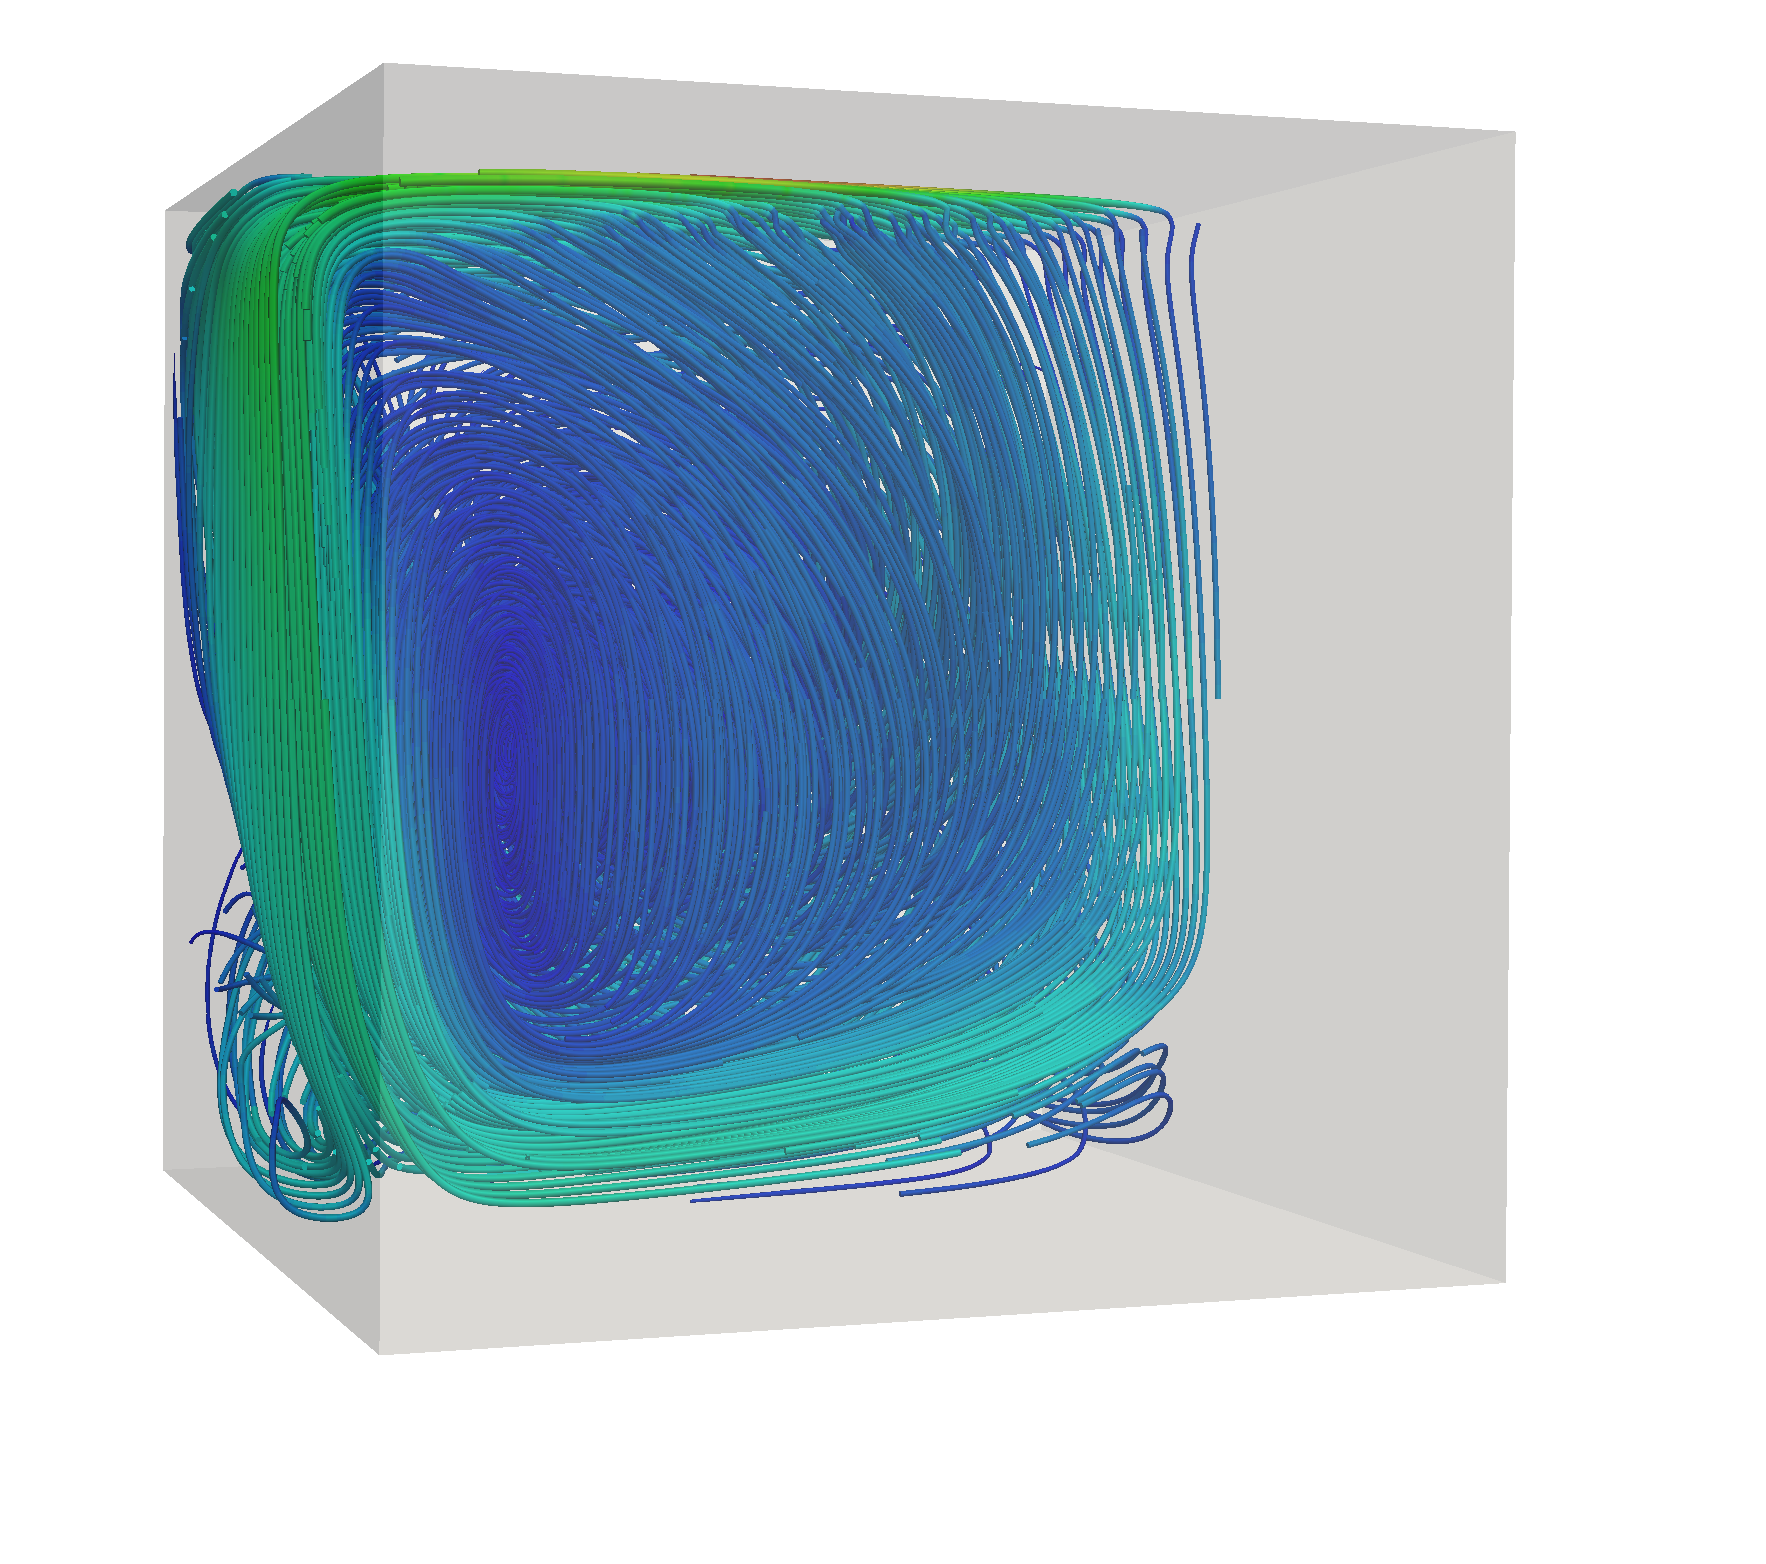
\includegraphics[height=4cm]{LDC-streamlines}\par}
    \end{minipage}

    {\raggedleft\small Details in \texttt{arXiv: 1810.03315 [math.NA]}\par}
  \end{posterbox}
  \begin{posterbox}[below=examples, name=details, column=4, span=2, height=0.14]{Want to know more?}
    \begin{minipage}[t]{0.85\textwidth}
      {\raggedright Paper: \texttt{arXiv: 1912.08516 [cs.MS]}\\
      Available in PETSc: \url{www.mcs.anl.gov/petsc}\\
      Interface in Firedrake: \url{www.firedrakeproject.org}\\
      Funding: EPSRC grants \texttt{EP/R029423/1},
      \texttt{EP/L015803/1}, \texttt{EP/N032861/1}\\
      \phantom{Funding:} U.S. DoE grant \texttt{DE-AC02-06CH11357}\par}
    \end{minipage}
    \begin{minipage}[t]{0.14\textwidth}
      \strut\vspace*{-\baselineskip}\newline
      {\centering 
\includegraphics[width=\textwidth]{pcpatch-paper-qr}\par}
    \end{minipage}

  \end{posterbox}
\end{poster}
\end{document}
